% ****** Start of file apssamp.tex ******
%
%   This file is part of the APS files in the REVTeX 4.2 distribution.
%   Version 4.2a of REVTeX, December 2014
%
%   Copyright (c) 2014 The American Physical Society.
%
%   See the REVTeX 4 README file for restrictions and more information.
%
% TeX'ing this file requires that you have AMS-LaTeX 2.0 installed
% as well as the rest of the prerequisites for REVTeX 4.2
%
% See the REVTeX 4 README file
% It also requires running BibTeX. The commands are as follows:
%
%  1)  latex apssamp.tex
%  2)  bibtex apssamp
%  3)  latex apssamp.tex
%  4)  latex apssamp.tex
%
\documentclass[%
 reprint,
%superscriptaddress,
%groupedaddress,
%unsortedaddress,
%runinaddress,
%frontmatterverbose,
%preprint,
%preprintnumbers,
%nofootinbib,
%nobibnotes,
%bibnotes,
 amsmath,amssymb,
 aps,
%pra,
%prb,
%rmp,
%prstab,
%prstper,
%floatfix,
]{revtex4-2}

\usepackage{graphicx}% Include figure files
\usepackage{dcolumn}% Align table columns on decimal point
\usepackage{bm}% bold math
\usepackage{bbm}
\usepackage{amsthm}

\usepackage{xcolor}
%\usepackage{hyperref}% add hypertext capabilities
%\usepackage[mathlines]{lineno}% Enable numbering of text and display math
%\linenumbers\relax % Commence numbering lines

%\usepackage[showframe,%Uncomment any one of the following lines to test
%%scale=0.7, marginratio={1:1, 2:3}, ignoreall,% default settings
%%text={7in,10in},centering,
%%margin=1.5in,
%%total={6.5in,8.75in}, top=1.2in, left=0.9in, includefoot,
%%height=10in,a5paper,hmargin={3cm,0.8in},
%]{geometry}
\newtheorem{theorem}{Theorem}[section]
\newtheorem{corollary}[theorem]{Corollary}
\newtheorem{proposition}[theorem]{Proposition}
\newtheorem{conjecture}[theorem]{Conjecture}
\newtheorem{claim}[theorem]{Claim}
\newtheorem{lemma}[theorem]{Lemma}
\newtheorem{remark}[theorem]{Remark}
\newtheorem{question}[theorem]{Question}
\newtheorem{definition}[theorem]{Definition}
\newtheorem{example}[theorem]{Example}
\newtheorem{problem}[theorem]{Problem}

\def\P{\mathbb{P}}
\def\N{\mathbb{N}}
\def\Z{\mathbb{Z}}
\def\Q{\mathbb{Q}}
\def\E{\mathbb{E}}
\def\R{\mathbb{R}}
\def\Var{\mathrm{Var}}
\def\Cov{\mathrm{Cov}}
\def\erf{\text{erf}}
\def\L{\mathcal{L}}
\def\F{\mathcal{p}}
\def\G{\mathcal{G}}
\def\sgn{\text{sgn}}
\def\bSigma{\boldsymbol{\Sigma}}
\def\bmu{\boldsymbol{\mu}}
\def\btheta{\boldsymbol{\theta}}
\def\btheta{\boldsymbol{\theta}}
\def\ybold{\mathbf{y}}
\def\xbold{\mathbf{x}}
\def\zbold{\mathbf{z}}
\def\sbold{\mathbf{s}}
\def\Rbold{\mathbf{R}}
\def\tr{\text{tr}}
\def\qhalf{q_{\left(\frac{1}{2}\right)}}
\def\Nacc{N_{\text{acc}}}
\def\Npos{N_{\text{pos}}}
\def\AECB{A_{\text{ECB}}}
\def\alphaECB{\alpha_{\text{ECB}}}
\def\Omegap{\Omega_{\text{p}}}
\def\fp{p_{\text{p}}}
\def\rb{r_{\text{b}}}
\def\fref{p_{\text{ref}}}
\newenvironment{sproof}{%
  \renewcommand{\proofname}{Sketch Proof}\proof}{\endproof}
\renewcommand{\d}{{\bf d}}
\newcommand{\btheta}{\mbox{\boldmath $\theta$}}
\newcommand{\bnu}{\mbox{\boldmath $\nu$}}
\newcommand{\e}{{\rm e}}


\begin{document}

\preprint{APS/123-QED}

\title{Fast evidence estimates of gravitational wave models via the Fourier integral method}
%\title{Using Fourier integral theorem for calculating\\the evidence of parametric gravitational wave models}% Force line breaks with \\
%\thanks{A footnote to the article title}%

\author{Siyang Li$^{1}$,  Patricio Maturana Russel$^{1,2}$, Renate Meyer$^1$, Avi Vajpeyi$^1$, and Guillaume Boileau$^3$}
\affiliation{$^1$ Department of
  Statistics, University of Auckland, Auckland 1142, New Zealand \\
$^2$ Department of Mathematical Sciences, \\Auckland University of Technology, New Zealand\\
$^3$ Universiteit Antwerpen, \\Prinstraat 13, 2000 Antwerpen, Belgium}

% Comments
\newcommand{\pmr}[1]{\textcolor{purple}{[PMR: #1]}}
\newcommand{\jason}[1]{\textcolor{blue}{[jason: #1]}}
\newcommand{\avi}[1]{\textcolor{orange}{[Avi: #1]}}
\newcommand{\todo}[1]{\textcolor{olive}{TODO: #1}}
\newcommand{\citeme}{\textcolor{purple}{(cite)}}



\date{\today}% It is always \today, today,
             %  but any date may be explicitly specified

\begin{abstract}
Abstract: a super fast method
\end{abstract}

\keywords{Fourier integral theorem, marginal likelihoods, gravitational wave models}%Use showkeys class option if keyword
                              %display desired
\maketitle

%\tableofcontents

\section{\label{sec:introduction} Introduction}
On September 14, 2015, the Laser Interferometer Gravitational-Wave Observatory (LIGO) directly detected gravitational waves for the very first time. These waves were emitted by the inspiral and merger of two solar mass black holes. For this spectacular discovery, the founders of LIGO, Barry Barish, Kip Thorne and Rainer Weiss were awarded the Nobel Prize in Physics in 2017.  Since then, the collaborations of the American LIGO detectors and the European Virgo detector have announced a total of 90 detections of gravitational waves (GWs) emitted by merging compact objects. LIGO, Virgo, and the Japanese KAGRA detector started another observation run in May 2023, which will last for 18 months and observe in the 20Hz to 2 kHz frequency range. The GWs observed to date stem from the mergers of solar-mass binary black holes and/or neutron stars but GWs from core-collapse supernovae and rapidly rotating neutron stars are potential sources that emit GWs in the frequency band of LIGO/Virgo/KAGRA (LVK).
Further ground-based interferometers with increased sensitivity, the Einstein Telescope in Europe and Cosmic Explorer in the US, are in the planning stages and should start observing in the mid 2030s. The Laser Interferometer Space Antenna or short LISA, a space mission led by the European Space Agency with support from NASA, and the Chinese space mission Tianji will observe in the mHz band from 2035 and will be sensitive to emissions from supermassive black holes, massive compact objects orbiting a supermassive black hole and the stochastic gravitational wave background from physical processes in the very early Universe.

To fully exploit the current and future observations and derive important information about the physics of the emitting sources, state-of-the-art statistical inference techniques are essential. To claim a detection with confidence requires a careful consideration of the evidence of the model with gravitational wave signal present as compared to a model with just instrumental noise. Furthermore, the observations of gravitational waves by terrestrial detectors now and by future space-based detectors present possibilities to put general relativity to the test. These require a methodology for statistical hypothesis tests or model comparison, e.g.\ testing the null hypothesis ``$H_0: M_0\mbox{ holds}$" against the alternative ``$H_1: M_1 \mbox{ holds}$".  Using a frequentist approach, hypothesis testing is done by
choosing a test statistic and calculating the so-called
p-value, the probability to reject the null hypothesis even if $M_0$ is true, see e.g.\ \cite{alma9998701914002091}. The p-value is usually regarded as an {\em indirect} measure of
the evidence against a null hypothesis (in favour of $M_1$) and often compared to the significance level of 5\%, i.e., if the p-value is larger
than 0.05, there is deemed to be insufficient evidence against the null hypothesis. However, the p-value cannot be interpreted (as often falsely done) as the probability that the null hypothesis is true. The p-value does not have this {\em direct} interpretation as a measure of evidence. This is only possible using a Bayesian approach by calculating the {\em evidence} for each model (insert citation), i.e., the marginal likelihood of the data $\ybold$ under model $M_i$, \[Z(M_i)=\pi(\ybold|M_i)=\int \pi(\btheta
_i|M_i)L(\ybold|\btheta_i,M_i)d\btheta_i.\]
This is the prior-weighted average of the likelihood of the data $\ybold$ given all potential parameter values $\btheta_i$ of Model $M_i$.
If the Bayes factor, defined as the ratio of the evidences,
\[ B_{01}=\frac{\pi(\ybold|M_0)}{\pi(\ybold|M_1)},\]
is larger than 1, this provides evidence in favour of $M_0$. Since $\pi(\ybold|M_i)=\pi(M_i|\ybold)\pi(M_i)$,
the Bayes factor can also be interpreted as the ratio of the posterior odds for model $M_0$, $\pi(\ybold|M_0)$, to the prior odds, $\pi(M_0)$.

However, apart from conjugate and low-dimensional cases, it is notoriously difficult to compute the marginal likelihood since it requires the solution of a high-dimensional integration problem.

A comprehensive overview of computational techniques for computing the marginal likelihood can be found in
\cite{RobertCP2009CmfB, GelmanAndrew2014, ChristensenNelson2022Pewg}.
Currently, the most widely-accepted methods for computing marginal likelihoods for gravitational wave data are nested sampling (NS) \cite{skilling2006nested, veitch2010bayesian}, thermodynamic integration (TI) \cite{gelman1998simulating, lartillot2006computing} and stepping-stone algorithm (SS) \cite{xie2011improving, maturana2019stepping}. These algorithms have been and are currently routinely used for LVK data analysis. All these use Monte Carlo samples from each model to estimate the evidence. A different approach is the transdimensional reversible jump Markov chain Monte Carlo method \cite{green1995reversible, umstatter2005bayesian} that explores the joint space of all models at once, and ratios of marginal likelihoods can be computed based on the proportions of the number of iterations that the algorithm stays in each model.
To circumvent the highdimensional integration, information criteria are often used for model comparison.
Under certain regularity conditions, an approximation to $-2\log Z$ is given by the frequentist Bayesian information criterion (BIC), defined as $\mbox{BIC}=-2\log L(\ybold|\hat{\btheta}) +p\log n$,
where $\hat{\btheta}$ denotes the maximum likelihood estimate, $p$ the number of parameters, and $n$ the sample size. This combines a measure of fit, the deviance $D(\btheta)= -2\log L(\ybold|\btheta)$ evaluated at the maximum likelihood estimate, with a penalty term for model complexity. A Bayesian version, the deviance information criterion (DIC, \cite{spiegelhalter2002bayesian}) uses
\[\mbox{DIC}=\bar{D}(\btheta) +p_D \]
with the posterior mean of the deviance $\bar{D}(\btheta)$  as the measure of fit and $p_D=\bar{D}(\theta)-D(\bar{\btheta})$ as the penalty term, where $\bar{\btheta}$ is the posterior mean of $\btheta$. The main advantages of using the DIC for model comparison is that it is easy to compute when a sample of the posterior distribution is available and that it can be used even if improper priors are specified. In contrast, Bayes factors cannot be interpreted if improper priors are used.


Here we propose the use of the Fourier integral method (FI) for computing the evidence of  gravitational wave models, as introduced by \cite{rotiroti2022computing}. It falls in the same category as nested sampling, the TI and SS algorithms in that no trans-dimensional moves are made nor information criteria used.
We aim to assess the accuracy and computational effort of the FI method in relation to these currently utilized techniques for computing the Bayes factor. This evaluation specifically focuses on LVK observations, with the goal of determining the evidence supporting the existence of a gravitational wave signal originating from a binary coalescence in LVK measurements.
The DIC has been employed in prior studies to assess gravitational wave models with and without phase transition in the context of the stochastic gravitational wave background (SGWB) based on simulated LISA observations \cite{BoileauGuillaume2023PfLt}. To demonstrate the comparative effectiveness of model comparison using the FI method in contrast to the DIC, we examine identical simulated data as presented in \cite{BoileauGuillaume2023PfLt}.

Computing the evidence through the Fourier integral method differs from methods like parallel tempered techniques (TI or SS) or sampling from progressively restricted parameter spaces like NS. The process does not necessitate these complexities. As long as there is knowledge of the prior and likelihood, along with a sample from the posterior distribution obtained, for instance, through a Metropolis-Hastings algorithm, implementing the Fourier integral method is notably straightforward and convenient. As far as the computation time is concerned,  the Fourier integral method is much faster than NS, TI and SS.  It is even  surpasses the computational speed of calculating the DIC. {\em What about accuracy?} As a consequence,
FI provides an accurate and fast alternative to current techniques and even compares favourably in terms of computation time to the calculation of information criteria.

The paper is structured as follows.... (delete the rest)

\bigskip

%%%%%%%%%%%%%%%%%%%%%%%%%%%%%%%%%%%%%%%%%%%%%%
Gravitational wave (GW) detection is a recent field in observational-based astronomy, which are waves of the gravitational field generated by perturbations of large masses in the universe. Ground-based detectors of gravitational waves include Laser Interferometer Gravitational-Wave Observatory (LIGO), Virgo interferometer and Kamioka Gravitational Wave Detector (KAGRA). However, GWs are detected by changes in distances between two points in the space-time, where such changes have tiny magnitudes on Earth. As a result, the LIGO-Virgo-KAGRA collaboration (LVK) is essential to increase the sensitivity and confidence of any GW signal detection.

Ground-based detectors can be spacious and prone to false signals due to human activities on the ground. The Laser Interferometer Space Antenna (LISA) will be a GW detector that will be sent into space, making it have high sensitivity to the millihertz GW frequency range. As stated in \cite{boileau2023prospects}, LISA will receive signals from various astronomical and cosmological sources.
%{\em Remark: Add general intro to LVK and LISA.}

Bayesian inference is currently the most widely adopted framework of inferences in astrophysics \cite{saha1994unfolding}, gravitational wave analysis \cite{christensen1998markov} and cosmology \cite{christensen2001bayesian, knox2001age}. When deciding which model better suits one data set, it is essential to conduct Bayesian model selection. In particular, gravitational waves are detected in the form of mixtures of waves emitted from various sources. Bayesian model selection processes are crucial in deciding which components exist in gravitational waves detected by LVK and LISA, which can be helpful in observing astronomical phenomenons that were not detected by gravitational waves. {\em Remark: Expand on the importance of model comparison for LVK/LISA. f}

There are various approaches to Bayesian model selection. The most fundamental approach is to compute and compare the evidence, also known as the marginal likelihood, of each model under consideration. However, the evidence is the integral of the posterior kernel function over the entire parameter space, which is often hard to compute when the parameter space is of high dimension. In addition, for the evidence to be defined, it is necessary for the prior distribution to be proper. This requirement is a drawback of Bayesian model selection based on the evidence since such a requirement stops the method from being applied to models with improper priors.
%{\em Remark: Expand a bit more: prior needs to be proper etc.}
%{\em Remark: I would put RJMCMC under computation of evidence, not a separate method for model comparison.}
A computationally convenient alternative to computing the evidence is model comparison via some information criterion, e.g.\ the deviance information criterion (DIC) \cite{spiegelhalter2002bayesian} that combines the model fit and complexity. {\em Expand a bit: here the focus is on evidence computation. next paragraph discusses the current computational techniques for computing the evidence. }

Currently, the most widely-accepted methods for computing marginal likelihoods for gravitational wave data are nested sampling (NS) \cite{skilling2006nested, veitch2010bayesian}, thermodynamic integration (TI) \cite{gelman1998simulating, lartillot2006computing} and stepping-stone algorithm (SS) \cite{xie2011improving, maturana2019stepping}. Another approach is the transdimensional reversible jump Markov chain Monte Carlo method \cite{green1995reversible, umstatter2005bayesian} that explores the joint space of all models at once, and ratios of marginal likelihoods can be computed based on the proportions of time of parameter space that the algorithm stays at. Here we propose the use of the Fourier integral method (FI) for computing the evidence of  gravitational wave models, as introduced by \cite{rotiroti2022computing}. We will compare the accuracy and computational effort of the FI method to those of the currently employed techniques for the calculation of the Bayes factor, the ratio of marginal likelihoods, to ascertain the evidence for the presence of a gravitational wave signal from a binary coalescence for LVK measurements. The DIC has previously been used to compare gravitational wave models with and without phase transition in the stochastic gravitational wave background (SGWB) for simulated LISA observations \cite{BoileauGuillaume2023PfLt}. To illustrate how model comparison via the FI compares to that of the DIC, we analyse the same simulated data as in \cite{BoileauGuillaume2023PfLt}.

{\em Remark: Finish with a summary of conclusions about FI.}
Evidence computation via the Fourier integral method only requires a good sample from the posterior distribution and the posterior kernel function to be known, and FI is also super convenient to implement. When the posterior sample size is large enough, with high accuracy, the Fourier integral method's computation time is much faster than that of NS, TI and SS, and it can also be thousands of times faster than computing the DIC. As a consequence,
FI provides an accurate and fast alternative to current techniques and even compares favourably in terms of computation time to the calculation of information criteria.
%with FI in use, the computation of  gravitational wave model evidence is never so fast, which can even erase the necessity of relying on DIC in some cases.

The paper is structured as follows. In Sec. \ref{sec:FI derivation} we discuss the derivation and mathematical properties of the Fourier integral method. In Sec. \ref{sec:simulation study} we compare the performance of the Fourier integral method with that of thermodynamic integration and stepping-stone algorithm in a simulation study. The performance of Fourier integral, nested sampling, thermodynamic integration, and stepping-stone are then compared with each other under LIGO merger data in Sec. \ref{sec:LIGO}. In Sec. \ref{sec:LISA} we apply the Fourier integral method to simulated LISA stochastic gravitational wave data and test if the conclusion is consistent with that using DIC. Finally, a summary discussion is given in Sec. \ref{sec:discussion}.

%{\em Remark: The paper is structured as follows...}

\section{\label{sec:FI derivation} The Fourier Integral Method}
%
\avi{We need to discuss (1) FI equation, (2) Selection of R, (3) selection of reference point.}



\avi{I think we should use GW community notation, ie $p(\theta|d) = \mathcal{L}(d|\theta) \pi(\theta) / \matcal{Z}(d)$}

In this section, we introduce the notation and provide an explanation of the FI method. Let $\d$ denote the observed data, e.g.\ a vector of GW measurements consisting of a GW strain signal embedded in noise:
\[d(t)=h(t|\btheta) + n(t),\quad t=1,\ldots,T, \]
where $\btheta=(\theta_1,\ldots,\theta_p)$ denotes the unknown parameters  that the GW strain signal $h(t|\theta)$ depends on, and $n(t)$ instrumental noise at time $t$.
To infer the unknown $\btheta$ within the Bayesian framework, we start with a prior distribution $\pi(\btheta)$ on the $p$-dimensional parameter space $\Theta$ and update this to the posterior distribution given the observations via Bayes' theorem
\begin{equation}\label{eq:Bayes}
  p(\btheta|\,\d)=\mathcal{L}(\d|\,\btheta) \pi(\btheta) / \matcal{Z}(\d)
 \end{equation}
where $\mathcal{L}(\d|\btheta)$ is the likelihood function, i.e.\ the joint probability density function of the data given parameter vector $\btheta$. Note that the denominator \[\matcal{Z}(\d)=\int_{\Theta} \mathcal{L}(\d|\,\btheta) \pi(\btheta) d\btheta\]
is the {\em marginal likelihood} or {\em evidence} of the GW model. This high-dimensional integral does not have an analytic
solution, in general, and numerical methods are required
for its calculation.

We now provide the underlying  idea of the FI method for calculating the evidence. By inverting Bayes' theorem (\ref{eq:Bayes}) one obtains
\begin{equation} \label{eq:invertedBayes}
 \matcal{Z}(\d) = \frac{\mathcal{L}(\d|\,\btheta) \pi(\btheta)}{p(\btheta|\,\d)}
 \end{equation}
which holds for any $\btheta\in \Theta$.
Provided that we have an estimate $\hat{p}$ of the posterior, e.g.\ in terms of a large sample, then we only need to be able to evaluate this at some chosen point $\btheta^*$ to obtain an estimate of the evidence:
\begin{equation}\label{eq:estimatedevidence}
\hat{\matcal{Z}}(\d) =  \frac{\mathcal{L}(\d|\,\btheta^*) \pi(\btheta^*)}{\hat{p}(\btheta^*|\,\d)}
\end{equation}
assuming that we can evaluate the likelihood and prior at $\btheta^*$.
This approach to computing the evidence was already suggested by \cite{chib1995marginal} and \cite{chib2001marginal}. Equation \eqref{eq:estimatedevidence} converts the problem of estimating the marginal likelihood, i.e., computing a multidimensional integral, into estimating the posterior density at one point in the parameter space.

The remaining problem is how to evaluate the posterior density when only an un-normalised posterior kernel is known. \cite{rotiroti2022computing} proposed a simple method that uses the well-known  Fourier integral theorem \cite{pristley2005introduction}. Suppose the posterior density $p$ is continuous and is defined over the entire $\R^d$.  For parameter vectors $\bnu$
and $\btheta$, let $\bnu \cdot \btheta=\sum_{i=1}^p \nu_i\theta_i$ denote the dot product and $\Rbold=(R_1,\ldots,R_p)$. Then the Fourier transform of the posterior $p$ is given by
\[
 \tilde{p}(\bnu|\d)=\int_{\R^p} p(\btheta|\,\d) \e^{-i\,\bnu\cdot\btheta} d\btheta
\]
and the Fourier inversion formula or Fourier integral theorem yields
\[p(\btheta^*|\,\d)= \left(\frac{1}{2\pi}\right)^p \int_{\R^P} \tilde{p}(\bnu|\d)\e^{i\,\btheta^*\cdot\bnu} d\bnu.\]
This can be expressed as the following limit:
\begin{eqnarray*}
p(\btheta^*|\,\d) &=& \left(\frac{1}{2\pi}\right)^p   \int_{\R^p} \left[ \int_{\R^p} p(\btheta|\,\d) \e^{-i \bnu \cdot \btheta} d\btheta\right]
 \e^{i\,\btheta^*\cdot\bnu} d\bnu\\
 &=& \left(\frac{1}{2\pi}\right)^p     \int_{\R^p}  \int_{\R^p} p(\btheta|\,\d) \e^{-i \bnu \cdot \btheta}
 \e^{i\btheta^*\cdot\bnu} d\bnu d\btheta\\
 &=& \left(\frac{1}{2\pi}\right)^p    \lim_{\Rbold\rightarrow \infty} \int_{\R^p}  \int_{-\Rbold}^{\Rbold} \cos\left(\bnu\cdot(\btheta^*-\btheta) \right)d\bnu p(\btheta|\d)   d\btheta\\
 &=& \frac{1}{\pi^p}   \lim_{\Rbold\rightarrow \infty} \int_{\R^p}  \prod_{j=1}^p \int_{0}^{R_j} \cos\left(\nu_j\cdot(\theta_j^*-\theta_j) \right)d\nu_j p(\btheta|\d)   d\btheta\\
 &=& \frac{1}{\pi^p}  \lim_{\Rbold\rightarrow \infty} \int_{\R^p}   \prod_{j=1}^p \frac{\sin\left(R_j(\theta_j^*-\theta_j) \right)}{\theta_j^*-\theta_j} p(\btheta|\d)   d\btheta
\end{eqnarray*}
Now, if we have a MCMC sample $\btheta^{(i)}$, $i=1,\ldots,n$, from the posterior distribution of $\btheta$, then the posterior at $\btheta^*$ can be estimated by
\begin{equation}\label{eq:estimatedpost}
\hat{p}_\text{FI}(\btheta^*|\,\d)=\frac{1}{n\pi^p} \sum_{i=1}^n \prod_{j=1}^p\frac{\sin\left(R_j(\theta_j^*-\theta_j^{(i)}) \right)}{\theta_j^*-\theta_j^{(i)}}
\end{equation}
for some fixed large $\Rbold$.
Plugging (\ref{eq:estimatedpost}) into (\ref{eq:estimatedevidence}) yields our Monte Carlo FI evidence estimate
\begin{equation}\label{eq:FIevidence}
 \hat{\matcal{Z}}_\text{FI}(\d) = \frac{\mathcal{L}(\d|\btheta^*)
 \pi(\btheta^*)}{\hat{p}_\text{FI}(\btheta^*|\d)}.
 \end{equation}
For practical applications of the FI evidence estimate, several questions remain:
\begin{enumerate}
     \item What is its bias and variance?
    \item How to choose $\btheta^*$?
    \item How to choose $\Rbold$?
    \item How to deal with a constrained parameter spaces $\Theta \subset \R^p$?
\end{enumerate}
These will be addressed in the subsequent subsections.


\subsection{\label{subsec:FI bias and variance} Bias and variance}
%
As shown in section 3.2 of \cite{rotiroti2022computing}, in the univariate case the bias and variance of $\hat{p}_\text{FI}(\btheta^*|\,\d)$ is at most of order $1/R$ and  $R/n$, respectively. For $d$-dimensional parameter spaces with a common value $R$ for all dimensions, the bias and variance is at most of order $1/R^d$ and  $R^d/n$, respectively. Typically, the bias is much smaller than $\frac{1}{R}$ as it depends on the differentiability and integrability of the posterior. For a Gaussian density or a mixture of Gaussian densities, the bias is of order $\e^{-R^2/2}$ \cite{rotiroti2022computing}. So for posterior distributions that are well approximated by a Gaussian or mixture of Gaussian distributions, the bias is very small.

The bias and variance of the FI estimator compare favourably with that of a kernel density estimator. The bandwidth $h$ of a kernel density estimator is a smoothing parameter. The bias and variance of the kernel density estimator is of order $h^2$ and $\frac{1}{nh}$, respectively, in the one-dimensional case.  With $R=1/h$ playing the role of the reciprocal of the smoothing parameter, the variance of both methods is of the same magnitude but the bias for the FI estimate is much smaller.

\subsection{\label{subsec:thetastar} Choice of $\btheta^*$}
In theory, the expression for the evidence in equation (\ref{eq:FIevidence}) holds for any point in the parameter space. However, for practical purposes, points with high posterior density should yield more efficient estimates \cite{chib1995marginal,chib2001marginal}. We recommend choosing the sample posterior mean or median for $\btheta^*$.

\textcolor{red}{Renate: I got up to here}
\vspace{4cm}


%%%%%%%%%%%%%%%%%%%%%%%%%%%%%%%%%%%%%%%%%%%%%%%%%%%%%%%%%%%%
% Jason's previous version
%%%%%%%%%%%%%%%%%%%%%%%%%%%%%%%%%%%%%%%%%%%%%%%%%%%%%%%%%%%%

\pmr{The Bayes' theorem is given by
\begin{equation} \label{eqn: Bayes' Theorem}
    p(\btheta |\ybold) = \frac{L(\btheta|\ybold)\pi(\btheta)}{c} =
    \frac{q(\btheta)}{c},
\end{equation}
where $\btheta \in \Theta$ denote the parameter vector, $\ybold$ the data, $L(\btheta|\ybold)$ the likelihood function, $\pi(\btheta)$ the prior density, assumed to be proper, i.e., $\int_\theta \pi(\btheta) d\btheta = 1$, $p(\btheta |\ybold)$ the posterior density, and where
\begin{equation} \label{eqn: posterior kernel q}
    q(\btheta) = L(\btheta|\ybold)\pi(\btheta)
\end{equation}
is the kernel of the posterior distribution, and
\begin{equation} \label{eqn: marginal likelihood}
    c = \int_\Theta L(\btheta|\ybold) \pi(\btheta) d\btheta
\end{equation}
is the marginal likelihood that quantifies the probability (density) of the appearance of the data that we observe.}

\subsection{\label{subsec:FI density estimation} Evidence computation via FI}

%Let the prior distribution $\pi(\btheta)$ be proper such that it is integrable and $\displaystyle \int_\Omega \pi(\btheta) d\btheta = 1$. Let $\ybold$ be the data being observed. Let $\btheta$ denote the parameter (vector) indexing the densities that can be expressed as (joint) likelihood functions, which have an unbounded support $\Omega$. Then for the prior distribution, likelihood function $L(\btheta|\ybold)$ and the posterior distribution $\pi(\btheta|\ybold)$, Bayes' Theorem says
%\begin{equation} \label{eqn: Bayes' Theorem}
%    \pi(\btheta|\ybold) = \frac{\pi(\btheta)L(\btheta|\ybold)}{p(\ybold)} =
%    \frac{q(\btheta)}{\int_\Omega q(\btheta) d\btheta},
%\end{equation}
%where
%\begin{equation} \label{eqn: posterior kernel q}
%    q(\btheta) := \pi(\btheta)L(\btheta|\ybold)
%\end{equation}
%is the kernel of the posterior distribution, and
%\begin{equation} \label{eqn: marginal likelihood}
%    c := p(\ybold) := \int_\Omega \pi(\btheta)L(\btheta|\ybold) d\btheta = \int_\Omega q(\btheta) d\btheta
%\end{equation}
%is the marginal likelihood that quantifies the probability (density) of the appearance of the data that we observe.

The Fourier integral (FI) method of calculating marginal likelihoods does not belong to any one of importance sampling, path sampling or bridge sampling classes of methods discussed in the following two sections \pmr{will we discuss the other methods?}. The method is based on a simple idea originated from \cite{chib1995marginal}, discussed in \cite{chib2001marginal} and also mentioned in \cite{raftery1995hypothesis}. \pmr{The method only relies on posterior samples, like the harmonic mean estimator, but it yields reliable estimates at a non-significant extra computational cost, which makes it a very attractive method.}

Suppose we are able to evaluate the posterior density at a pre-chosen point $\mathbf{x} = (x_1, x_2, \ldots, x_d) \in \Theta$, then Bayes' theorem  defined in Equation \eqref{eqn: Bayes' Theorem} can be re-arranged as
\begin{equation} \label{eqn: re-arranged Bayes' Theorem for FI method}
    c = \frac{L(\xbold | \ybold)\pi(\xbold)}{p(\xbold | \ybold)}.
\end{equation}
%\begin{equation} \label{eqn: re-arranged Bayes' Theorem for FI method}
%    c = p(\ybold) = \frac{\pi(\xbold)L(\xbold | \ybold)}{\pi(\xbold | \ybold)},
%\end{equation}
%where $\xbold$ is a vector with a single value for each dimension of the parameter space.

% Note that, to clarify the difference between any arbitrary points in the parameter space $\theta$ and the specific pre-chosen point for the purpose of Fourier integral method, we denote the former by $\btheta$ and the later by $\xbold$. In addition, the parameter space is usually explored by the posterior sample, so the posterior sample is denoted by $\btheta^{(i)}$. In practice, $\btheta$ and $\xbold$ have different sources - $\btheta^{(i)}$ come from sampling from the posterior kernel function, whereas $\xbold$ comes from the researchers' minds, and that $\xbold$ will only have this meaning throughout this dissertation. Although both of them live in the same parameter space, it is important to bear the difference between $\btheta$ and $\xbold$ in mind, otherwise the final Fourier integral estimator can be very confusing. In practice, $\xbold$ is usually chosen to be the most convenient point for computation purposes, which could be $\mathbf{0}$ or the posterior mean. As discussed in \cite{chib1995marginal} and \cite{chib2001marginal}, points with higher density values should be more efficient in terms of density estimation.

\pmr{Equation \eqref{eqn: re-arranged Bayes' Theorem for FI method} converts the problem of estimating the marginal likelihood, i.e., a multidimensional integral calculation, into estimating the posterior density at one point in the parameter space. The remaining problem is how to evaluate the posterior density when only an un-normalised posterior kernel is known. \cite{rotiroti2022computing} proposed a simple method that uses the well-known Fourier transform.}

\pmr{To clarify the difference between any arbitrary points in the parameter space $\theta$ and the specific pre-chosen point for the purpose of Fourier integral method, we denote the former by $\btheta$ and the later by $\xbold$. Note that $\xbold$ is a vector with a single value for each dimension of the parameter space arbitrarily defined. It has been suggested that $\btheta$ with higher density values should be more efficient in terms of density estimation \citep{chib1995marginal, chib2001marginal}, making the posterior mean a popular choice.}
% In the following, $\btheta^{(i)}$ stand for the $i$th posterior sample.  In practice, $\btheta$ and $\xbold$ have different sources - $\btheta^{(i)}$ come from sampling from the posterior kernel function, whereas $\xbold$ is arbitrarily defined.


%Equation \eqref{eqn: re-arranged Bayes' Theorem for FI method} converts the problem of estimating marginal likelihoods (integrals) into estimating the posterior density at one point (no integration needed). The remaining problem is how to evaluate the posterior density when only an un-normalised posterior kernel is known. \cite{rotiroti2022computing} proposed a simple method that uses the well-known Fourier transform.

\pmr{We can probably define the method for the d-dimensional case, skipping d=1 case.}

Suppose the posterior density $p$ is continuous and is defined over the entire $\R^d$. \pmr{For simplicity, we omit the conditioning on the data $\ybold$.}  Then, the Fourier transform of $p$ is given by
\begin{equation} \label{eqn: fourier transform}
    \Tilde{p}(s) = \int_{-\infty}^\infty p(x) e^{-isx}dx,
\end{equation}
where $s \in \R$ is arbitrary and $i$ is the imaginary number such that $i^2 = -1$. The inverse of such a transformation can be found as
\begin{equation} \label{eqn: inverse Fourier transform}
    p(x) = \frac{1}{2\pi}\int_{-\infty}^\infty \Tilde{p}(s) e^{isx}ds,
\end{equation}
where $x \in \R$ is arbitrary \pmr{is this not the $\mathbf{x}$ defined above?}. The definition of Fourier transform and its inverse can be found in numerous textbooks in applied mathematics, such as \cite{pristley2005introduction}. Combining equations \eqref{eqn: fourier transform} and \eqref{eqn: inverse Fourier transform}, it can be shown that
\begin{align} \label{eqn: univariate Fourier integral}
    p(x) & = \frac{1}{2\pi}\int_{-\infty}^\infty \Tilde{p}(s) e^{isx}ds \\
    %& = \frac{1}{2\pi}\int_{-\infty}^\infty \left[\int_{-\infty}^\infty p(\theta) e^{-is\theta}d\theta\right] e^{isx}ds \\
    %& = \frac{1}{2\pi} \lim_{R \to \infty} \int_{-\infty}^\infty \int_{-R}^R \cos[s(x-\theta)]ds p(\theta)d\theta \\
    & = \frac{1}{\pi} \lim_{R \to \infty} \int_{-\infty}^\infty \frac{\sin[R(x-\theta)]}{x-\theta}p(\theta)d\theta \label{eq:fi_exp_post}
\end{align}
%as the function $p$ is real. Note that $\theta \in \R \equiv \Omega$ in this case, which means any arbitrary point in the parameter space. In addition, if $p$ is a proper density function, then the last line is equivalent to an expectation with respect to such a density. Consequently, we can let $p$ be the posterior density function $\pi(\cdot|\ybold)$ and use the posterior sample as the dummy variable $y$ such that
as the posterior is real. Note that $\theta \in \R \equiv \Omega$ in this case, which means any arbitrary point in the parameter space. Since $p$ is a proper density function, Equation~\eqref{eq:fi_exp_post} is equivalent to an expectation with respect to the posterior. Consequently, we can let $p$ be the posterior density function $\pi(\cdot|\ybold)$ and use the posterior sample as the dummy variable $y$ such that
\begin{align} \label{eqn: univariate Fourier integral density estimator}
    & \pi(x|\ybold) = \lim_{R \to \infty} E\left\{\frac{\sin[R(x-\theta)]}{x-\theta} \bigg|\ybold\right\} \implies \\ & \hat{\pi}_\text{FI}(x|\ybold) = \hat{p}_\text{FI}(x) = \frac{1}{n\pi}\sum_{i = 1}^n \frac{\sin(R(x - \theta^{(i)}))}{x - \theta^{(i)}}
\end{align}
where $R$ is any chosen large values in practice. Finally, we can plug equation \eqref{eqn: univariate Fourier integral density estimator} into the following equality inspired by equation \eqref{eqn: re-arranged Bayes' Theorem for FI method}:
\begin{equation} \label{eqn: re-arranged Bayes' Theorem for FI method estimator}
    \hat{c}_{FI} = \frac{\pi(\xbold)L(\xbold | \ybold)}{\hat{\pi}_n (\xbold | \ybold)},
\end{equation}
which gives a simple-yet-convincing estimator of the marginal likelihood $c$.

However, equation \eqref{eqn: univariate Fourier integral density estimator} only considers the case where the parameter space $\Omega$ is one-dimensional. Let  $d \in \N$ and $\infty^d$ denote a vector of infinity of length $d$. Let $\mathbf{s} \cdot \btheta$ denote the dot product for vectors $\mathbf{s}$ and $\btheta$. For $d$-dimensional parameter spaces, Fourier transformation and its inverse yield
\begin{align} \label{eqn: multivariate Fourier integral}
    p(\xbold) & = \left(\frac{1}{2\pi}\right)^d\int_{\R^d} \int_{\R^d}p(\btheta) e^{-i\sbold\btheta}d\btheta e^{i\sbold\xbold}d\sbold \\
    & = \left(\frac{1}{2\pi}\right)^d \lim_{\Rbold \to \infty^d} \int_{\R^d} \int_{-\Rbold}^\Rbold \cos[\sbold(\xbold-\btheta)]d\sbold p(\btheta)d\btheta \\
    & = \frac{1}{\pi^d} \lim_{\Rbold \to \infty^d} \int_{\R^d} \prod_{j=1}^d \int_0^{R_j} \cos[s_j(x_j-\theta_j)]ds_j p(\btheta)d\btheta \\
    & = \frac{1}{\pi^d} \lim_{\Rbold \to \infty^d} \int_{\R^d} \prod_{j=1}^d \frac{\sin[R_j(x_j-\theta_j)]}{x_j-\theta_j} p(\btheta)d\btheta
\end{align}
by linear independence of different dimensions of $\sbold := (s_1, s_2, \ldots, s_d)$ in the integral, and $\Rbold := (R_1, R_2, \ldots, R_d)$. Note that $\theta_j$ denotes the $j$-th dimension of the parameter vector $\btheta$. For $\Rbold$ being a vector of large constants and $p$ being a $d$-dimensional density function, one can thus observe an estimator of the density:
\begin{equation} \label{eqn: multivariate Fourier integral density estimator}
    \hat{p}_\text{FI}(\mathbf{x}) = \frac{1}{n\pi^d}\sum_{i = 1}^n \prod_{j = 1}^d \frac{\sin(R_j(x_j - \theta_j^{(i)}))}{x_j - \theta_j^{(i)}},
\end{equation}
where $\theta_j^{(i)}$ is the $i$-th data on dimension $j$ of the sample from function $p$; in other words, $\theta_j^{(i)}$ is the $j$-th dimension of the $i$-th observation in the multivariate sample from density $p$. In addition, $\mathbf{x} = (x_1, x_2, \ldots, x_d) \in \R^d$ is the pre-chosen point where the density function is evaluated. By considering $\hat{p}_n(\mathbf{x})$ in equation \eqref{eqn: multivariate Fourier integral density estimator} as the quantity $\hat{\pi}_n (\xbold | \ybold)$ in equation \eqref{eqn: re-arranged Bayes' Theorem for FI method estimator}, we can find the complete Fourier integral estimator for marginal likelihoods where the parameter space is high dimensional.

%%%%%%%%%%%%%%%%%%%%%%%%%%%%%%%%%%%%%%%%%

\subsection{\label{subsec:transformation of parameter space} Transformation of parameter space}
As defined by equation \eqref{eqn: fourier transform}, Fourier transform requires the function $p$ being transformed to be $f \in \mathcal{C}(\R)$; otherwise, the integrand in the integral of equation \eqref{eqn: fourier transform} is undefined at some parts to be integrated, or that there needs to be indicator functions and Dirac delta functions to take care of the discontinuity. When $p$ is the probability density of a distribution, such a function domain requirement means that the indicator function of the density support needs to be specified within $p$. When the support of $p$ is only part of the real space, it is usually discontinuous at the boundary of its support. This makes $p$ fail to meet the assumption at the beginning of section 3 in \cite{rotiroti2022computing}, hence making the bias and variance calculation in their section 3.2 not necessarily true.

A simple example is $\theta \sim \text{Exp}(\lambda)$; that is, $p_\theta(\theta) = \lambda e^{-\lambda \theta} \mathbbm{1}[\theta > 0]$. Then $p_\theta \notin \mathcal{C}(\R)$. As discussed at the beginning of section 3.2 of \cite{rotiroti2022computing}, the bias of $\hat{p}_n(x)$ is given by $\displaystyle \frac{I(R)}{\pi}$, where
\begin{align} \label{eqn: FI Exp bias}
    I(R) & = \int_{-\infty}^\infty \sin(R\theta) \frac{p_\theta(\theta) - p_\theta(0)}{\theta} d\theta \\
    %& = \lambda \int_{-\infty}^\infty \frac{\sin(R\theta)}{\theta} e^{-\lambda \theta} \mathbbm{1}[\theta > 0] d\theta - \lambda \int_{-\infty}^\infty \frac{\sin(R\theta)}{\theta} e^0 \mathbbm{1}[\theta > 0] d\theta \\
    & = \lambda \int_0^\infty \frac{\sin(R\theta)}{\theta} e^{-\lambda \theta} d\theta - \lambda \int_0^\infty \frac{\sin(R\theta)}{\theta} d\theta
\end{align}
The first integral in \eqref{eqn: FI Exp bias} can be calculated using a Laplace transform on the sinc function, and the second integral can be calculated by the sine integral function as in \cite{rotiroti2022computing}. In particular,
\begin{align} \label{eqn: FI Exp asymptotic}
    & \lambda \int_0^\infty \frac{\sin(R\theta)}{\theta} e^{-\lambda \theta} d\theta = \lambda \mathcal{L}\left\{\frac{\sin(R\theta)}{\theta} \right\} \\
    = & \lambda \arctan\left(\frac{R}{\lambda}\right) \sim R
\end{align}
and
\begin{equation} \label{eqn: FI Exp Dirichlet Integral}
    \lambda \int_0^\infty \frac{\sin(R\theta)}{\theta} d\theta = \lim_{k \to \infty} \lambda \int_0^k \frac{\sin(R\theta)}{\theta} d\theta = \lambda\frac{\pi}{2}.
\end{equation}
The mathematical details of equations \eqref{eqn: FI Exp asymptotic} and \eqref{eqn: FI Exp Dirichlet Integral} can be found in the appendix, section \ref{subsec: maths details of the FI Exp example}. Finally, by combining equations \eqref{eqn: FI Exp asymptotic} and \eqref{eqn: FI Exp Dirichlet Integral}, one gets, when $R \to \infty$
\begin{equation} \label{eqn: FI Exp bias I component}
    I(R) \sim R - \lambda \frac{\pi}{2} >> \frac{1}{R},
\end{equation}
so the bias in $\hat{p}_n(x)$ can be much larger than order $\frac{1}{R}$ when the parameter $\lambda$ is large enough. Here we propose a solution that uses change-of-variable technique on equation \eqref{eqn: re-arranged Bayes' Theorem for FI method}.
\begin{lemma} \label{lemma: FI transforming the re-arranged Bayes theorem}
    Suppose $g: x \mapsto \check{x} \in \R$ is an invertible transformation of parameter $x$. Let $q$ denote the posterior kernel function defined by equation \eqref{eqn: posterior kernel q}. Then
    \begin{equation*}
        c = \frac{q_{\check{x}}(\check{x}|\ybold)}{\pi_{\check{x}}(\check{x}|\ybold)}.
    \end{equation*}
\end{lemma}
\begin{proof}
    By the assumption in the lemma, $x = g^{-1}(\check{x})$. Starting from equation \eqref{eqn: re-arranged Bayes' Theorem for FI method}, we have
    \begin{align*}
        & \pi_x(x|\ybold) = \frac{q_x(x|\ybold)}{c} \\
        \implies & \pi_x(g^{-1}(\check{x})|\ybold) = \frac{q_x(g^{-1}(\check{x})|\ybold)}{c} \\
        \implies & \pi_{\check{x}}(\check{x}|\ybold) = \pi_x(g^{-1}(\check{x})|\ybold)|J| \\
        & = \frac{q_x(g^{-1}(\check{x})|\ybold)|J|}{c} = \frac{q_{\check{x}}(\check{x}|\ybold)}{c} \\
        \implies & c = \frac{q_{\check{x}}(\check{x}|\ybold)}{\pi_{\check{x}}(\check{x}|\ybold)},
    \end{align*}
    where $J$ stands for the Jacobian matrix in such a transformation of random variable.
\end{proof}
Intuitively, it is easy to understand lemma \ref{lemma: FI transforming the re-arranged Bayes theorem}, such that reparametrization of a model will never change the likelihood of a model, neither making the model more likely nor less likely. Consequently, by estimating $\pi_{\check{x}} \in \mathcal{C}(\R)$ rather than $\pi_x \notin \mathcal{C}(\R)$, one can largely reduce the bias due to $\Omega \neq \R^d$.

However, it is worth noting that, although the solution by lemma \ref{lemma: FI transforming the re-arranged Bayes theorem} can reduce the bias by transforming $\Omega$ to $\R^d$, the variance of such an estimate shall depend on the transformation $g$ and the values in the posterior sample. In practice, it is not uncommon to see increases in the variability of marginal likelihood estimates after the transformation.

\subsection{\label{subsec:relationship between FI and KDE} The relationship between FI and KDE}

One highlight of FI is that it considers the sine function as the kernel of density estimation in equations \eqref{eqn: univariate Fourier integral density estimator} and \eqref{eqn: multivariate Fourier integral density estimator}, unlike the usual uniform or Gaussian kernels. In fact, \cite{ho2021integral} discusses integral theorems in general, such that, in the density estimator
\begin{equation} \label{eqn: general integral theorem estimator}
    \hat{p}_R(\mathbf{x}) = \frac{1}{n\pi^d}\sum_{i = 1}^n \prod_{j = 1}^d \frac{\phi(R(x_j - \theta_j^{(i)}))}{x_j - \theta_j^{(i)}},
\end{equation}
the kernel $\phi$ only needs to be a cyclic function over the interval $(0, 2\pi)$, such that it integrates to 0 over $(0, 2\pi)$. Examples of integral theorems in \cite{ho2021integral} include the Haar wavelet integral theorem and Spline integral theorem, where each of them correspond to a unique density estimator, in a similar form of equations \eqref{eqn: univariate Fourier integral density estimator} and \eqref{eqn: multivariate Fourier integral density estimator}. Nevertheless, \cite{ho2021integral} showed that
\begin{equation} \label{eqn: optimal cyclic kernel (sine)}
    \phi(x) = \frac{\sin(x)}{\pi}
\end{equation}
is the optimal cyclic and almost everywhere differentiable kernel, such that it minimizes the mean integrated square error
\begin{equation} \label{eqn: mean integrated square error}
    \int_\R \left(\frac{\phi(x)}{x} \right)^2dx.
\end{equation}
As a result, \cite{ho2021integral} provides a method of generalizing FI.

However, considering different integral theorems is not the only way of generalizing FI. Considering how the integrals approach infinity will generalize FI in another way, yielding some well-known KDEs. Note that equation \eqref{eqn: univariate Fourier integral} can be reexpressed as
\begin{align*}
    p(x) & = \frac{1}{2\pi} \lim_{R \to \infty} \int_{-\infty}^\infty \int_{-R}^R \cos[s(x-\theta)]ds p(\theta)d\theta \\
    & = \frac{1}{2\pi} \lim_{R \to \infty} \int_{-\infty}^\infty \int_{-\infty}^\infty \\
    & \hspace{1cm}\cos[s(x-\theta)] \mathbbm{1}[-R < s < R] ds p(\theta) d\theta \\
    & = \frac{1}{2\pi} \lim_{R \to \infty} \int_{-\infty}^\infty \int_{-\infty}^\infty \cos[s(x-\theta)]h_R(s)ds p(\theta)d\theta
\end{align*}
where the integral window, $h_R(s) = \mathbbm{1}[-R < s < R]$, can be considered as the kernel of a Uniform$(-R, R)$ function. Furthermore, such a kernel is being put into a limit $R \to \infty$ that makes the uniform kernel converges to the constant function $h(s) = 1$. As a result, there are other sequences of functions that can replace $h_R(s) = \mathbbm{1}[-R < s < R]$ for the role of integral windows as long as they have the limit $h(s) = 1$, which gives the estimator different convergence behaviours. See figure \ref{fig:FI integral windows} for visual illustration of different types of functional sequences converging to $h(s) = 1$. We call $\epsilon$ in all kinds of $h_\epsilon(\theta)$ the `limiting factor', where such a limiting factor is not necessarily $R \to \infty$, but it can also be $\tau \to 0$, depending on the functional sequence.
\begin{proposition}
    The integral-window-generalized Fourier integral density estimating equation has the form
    \begin{equation} \label{eqn: integral window h(s)}
        p(x) = \frac{1}{2\pi} \lim_{\epsilon \to k(h)} \int_{-\infty}^\infty \int_{-\infty}^\infty \cos[s(x-\theta)]h_\epsilon(s)ds p(\theta)d\theta,
    \end{equation}
    where $k(h) \in \R \cup \{-\infty, \infty\}$ is the constant that the limiting factor $\epsilon$ should converge to, in order to guarantee $h_\epsilon(s)$ converges to $h(s) = 1$, and $\displaystyle\lim_{|s| \to \infty} h_\epsilon(s) = 0$ is necessary.
\end{proposition}

\begin{figure}
    \centering
    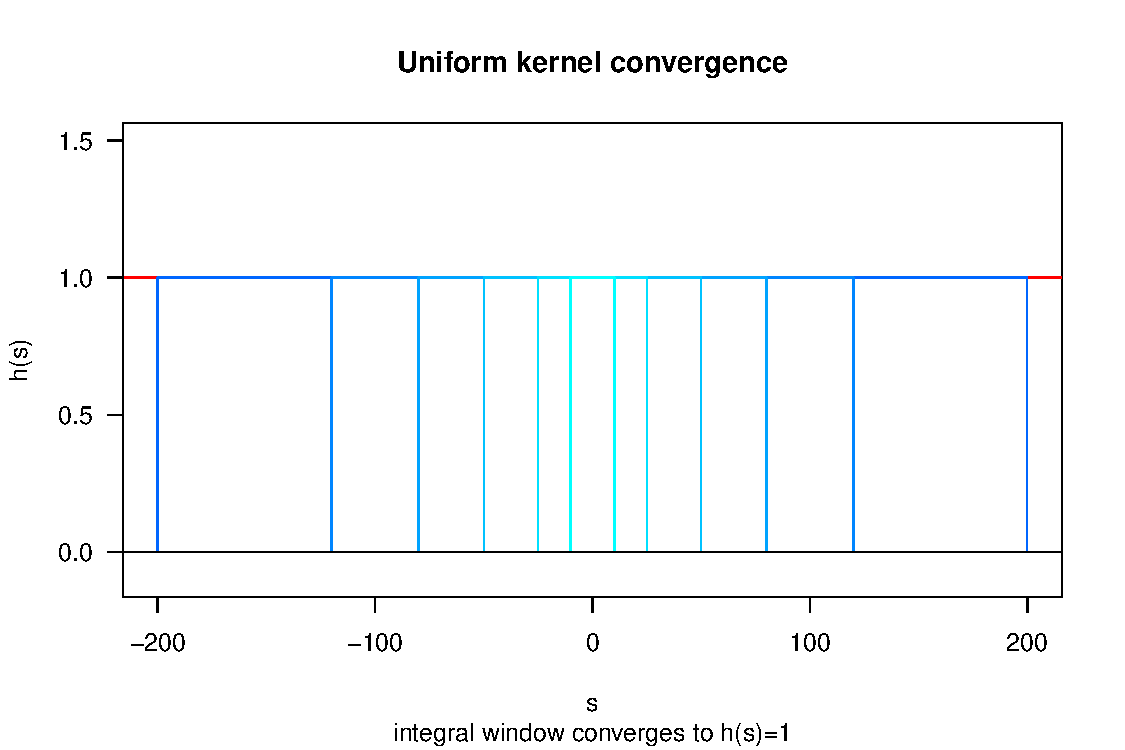
\includegraphics[page = 1, scale = 0.45]{pictures/section 2/integralwindow.pdf}
    \includegraphics[page = 2, scale = 0.45]{pictures/section 2/integralwindow.pdf}
    \caption{Different types of integral windows}
    \label{fig:FI integral windows}
\end{figure}

As a result, considering different functional sequences as the integral windows will give different estimators.The following theorem summarises the results by some natural choices of integral windows:

\begin{theorem} \label{theorem: FI integral windows}
For any reference point $x \in \Omega$, $\tau$ a small positive value and $R$ a fixed large constant:
    \begin{enumerate}
        \item Uniform kernel $h_R(s) = \mathbbm{1}[-R < s < R]$ in equation \eqref{eqn: integral window h(s)} leads to equation \eqref{eqn: univariate Fourier integral density estimator}.
        \item Normal kernel $h_\tau(s) = e^{-s^2\tau}$ in equation \eqref{eqn: integral window h(s)} leads to
        \begin{equation} \label{eqn: normal window FI}
            \hat{p}_n(x) = \frac{1}{n} \sum_{i = 1}^n p_\text{Norm}(\theta^{(i)}; \text{mean} = x, \text{var} = 2\tau).
        \end{equation}
        \item Double-exponential kernel $h_\tau(s) = e^{-|s|\tau}$ in equation \eqref{eqn: integral window h(s)} leads to \begin{equation} \label{eqn: Cauchy window FI}
            \hat{p}_n(x) = \frac{1}{n} \sum_{i = 1}^n p_\text{Cauchy}(\theta^{(i)}; \text{location} = x, \text{scale} = \tau).
        \end{equation}
        \item Triangular kernel $h_R(s) = (1 - \frac{|s|}{R}) \mathbbm{1}[-R < s < R]$ in equation \eqref{eqn: integral window h(s)} leads to
        \begin{equation} \label{eqn: triangular kernel window FI}
            \hat{p}_n(x) = \frac{1}{n\pi} \sum_{i = 1}^n \frac{1}{R(x - \theta^{(i)})^2}\{1 - \cos[R(x - \theta^{(i)})]\}.
        \end{equation}
        \item Epanechnikov kernel $h_R(s) = (1 - \frac{s^2}{R^2}) \mathbbm{1}[-R < s < R]$ in equation \eqref{eqn: integral window h(s)} leads to
        \begin{equation} \label{eqn: Epanechnikov kernel window FI}
            \hat{p}_n(x) = \frac{1}{n\pi} \sum_{i = 1}^n \frac{2\left\{\frac{\sin[R(x - \theta^{(i)})]}{x - \theta^{(i)}} - R\cos[R(x - \theta^{(i)})] \right\}}{R^2(x - \theta^{(i)})^2}.
        \end{equation}
    \end{enumerate}
\end{theorem}

In comparison, Gaussian KDE has the form
\begin{align} \label{eqn: Gaussian KDE}
    \hat{p}_h(x) & = \frac{1}{nh}\sum_{i = 1}^n \frac{1}{\sqrt{2\pi}}\exp\left[-\frac{1}{2}\left(\frac{|x - \theta^{(i)}|}{h} \right)^2 \right] \\
    & = \frac{1}{n}\sum_{i = 1}^n p_\text{Norm}(\theta^{(i)}; \text{mean} = x, \text{var} = h^2).
\end{align}
Therefore, by comparing equations \eqref{eqn: normal window FI} and \eqref{eqn: Gaussian KDE}, one can see that Gaussian KDE is identical to the integral-window-generalized FI estimator when $2\tau = h^2$, so we have derived KDE from FI. A similar result holds for the Cauchy-kernel KDE by investigating equation \eqref{eqn: Cauchy window FI}. This leads to the following result:

\begin{corollary}
Fourier integral estimator is a special case of kernel density estimator.
\end{corollary}

However, as claimed in section \ref{subsec:FI bias and variance} and in \cite{rotiroti2022computing}, FI is superior to ordinary KDE in many cases. On the other hand, estimators \eqref{eqn: triangular kernel window FI} and \eqref{eqn: Epanechnikov kernel window FI} follow the form of equation \eqref{eqn: general integral theorem estimator}, so they follow the result \cite{ho2021integral} that they are not as efficient as the sine kernel.

Another corollary of thinking about the integration windows is:
\begin{corollary} \label{corollary: FI estimators underestimate densities}
    $\forall n \in \N, \, \hat{p}_n(x) \le p(x)$. That is, FI estimates are always underestimates to the true underlying density $p(x)$.
\end{corollary}

This is easy to understand - only when the integral window is $h(s) = 1$, the FI estimators will equal to the true underlying value. Whenever the integral window only covers part of the area under $h(s) = 1$, the density will be underestimated, leading to overestimated $\hat{c}_\text{FI}$. However, as it is necessary to have $\displaystyle\lim_{|s| \to \infty} h_\epsilon(s) = 0$, it is impossible to have an unbiased FI estimator without any limiting factors.

Another aspect of the comparison between FI and KDE is via considering their discrete analogs. For any integrable $p$ defined on $[-\pi, \pi]$ where $p(-\pi) = p(\pi)$, the Fourier coefficients are
\begin{equation*}
    \underline{p}(n) = \frac{1}{2\pi}\int_{-\pi}^\pi p(\theta) e^{-in\theta}d\theta
\end{equation*}
in Fourier partial sums
\begin{equation*}
    S_N(f; \theta) = \sum_{n = -N}^N \underline{p}(n) e^{in\theta}.
\end{equation*}
Then for the Dirichlet kernel (see \cite{bhatia2005fourier})
\begin{equation*}
    D_N(t) = \frac{1}{2\pi} \sum_{n = -N}^N e^{int},
\end{equation*}
Fourier partial sums can be re-expressed as
\begin{align} \label{eqn: Dirichlet kernel Fourier partial sum}
    S_N(f; \theta) = & \frac{1}{2\pi} e^{in\theta} \sum_{n = -N}^N \int_{-\pi}^\pi p(t) e^{-int}dt\\
    = & \frac{1}{2\pi} \sum_{n = -N}^N \int_{-\pi}^\pi p(t) e^{in(\theta - t)}dt = (f \star D_N)(\theta),
\end{align}
which is mostly identical to the steps that derived FI, equation \eqref{eqn: univariate Fourier integral}. Therefore, FI corresponds to Dirichlet kernels. Similarly, for $r \in [0, 1)$, the Poisson kernel (see \cite{bhatia2005fourier})
\begin{equation*}
    P(r, \theta) = \frac{1}{2\pi} \frac{1-r^2}{1-2r\cos(\theta)+r^2}
\end{equation*}
is obtained by considering
\begin{equation} \label{eqn: Poisson kernel Fourier partial sum}
    u(r, \theta) = \frac{1}{2\pi} \sum_{n = -\infty}^\infty \int_{-\pi}^\pi r^{|n|} e^{in(\theta-t)} p(t)dt,
\end{equation}
which is mostly identical to equation \eqref{eqn: integral window h(s)} with the integral window $h_r(n) = r^{|n|}$, which is one case in KDE. Therefore, KDE corresponds to Poisson kernels.

As in \cite{bhatia2005fourier}, by Jordan's theorem, if $p$ is continuous and of bounded variation on $[-\pi, \pi]$, then equation \eqref{eqn: Dirichlet kernel Fourier partial sum} has $\displaystyle S_N(f; \theta) \to p(\theta)$ as $N \to \infty$ at every point where $p$ is continuous, and such a convergence is uniform on any closed intervals that do not contain a discontinuity of $p$. On the other hand, by Poisson's theorem, if $p$ is continuous on $[-\pi, \pi]$, then in equation \eqref{eqn: Poisson kernel Fourier partial sum}, $u(r, \theta) \to p(\theta)$ uniformly as $r \to 1$. Therefore, FI corresponds to the Dirichlet kernel that requires the underlying density $p$ to be continuous and of bounded variation, whereas KDE belongs to the Poisson kernel that only requires the underlying density to be continuous. This makes a difference in density estimations for nonparametric densities, where the shape of the density approaches a non-bounded-variation function in some regions. Consequently, KDE could work well for nonparametric densities, but FI may not.

\subsection{\label{subsec:comprehensive FI} A more comprehensive FI estimator}

One drawback of the sine (more generally, Dirichlet) kernel used in FI is that it may produce negative density estimates. This issue is usually more severe for parameter spaces with higher dimensions. Namely, $\sin(R(x - \theta^{(i)}))$ and $x - \theta^{(i)}$ can have opposite signs. For one specific observation $i$, if the total number of negative $\displaystyle \frac{\sin(R(x_j - \theta_j^{(i)}))}{x_j - \theta_j^{(i)}}$ is odd, then $\displaystyle \prod_{j = 1}^d \frac{\sin(R(x_j - \theta_j^{(i)}))}{x_j - \theta_j^{(i)}}$ will be negative. If the total magnitude of such negative values exceed the total magnitude of positive values out of the same quantity, then equation \eqref{eqn: multivariate Fourier integral density estimator} is negative. For each dimension $j$ of each observation $i$, it is very easy to calculate which $R$ values can give positive $\displaystyle \frac{\sin(R(x_j - \theta_j^{(i)}))}{x_j - \theta_j^{(i)}}$ analytically. When there is a second dimension for this observation $i$, the region for $R$ that gives positive $\displaystyle \prod_{j = 1}^2 \frac{\sin(R(x_j - \theta_j^{(i)}))}{x_j - \theta_j^{(i)}}$ is the union of where the fraction is positive for both dimensions, and where the fraction is negative for both dimensions. When the number of dimensions $d$ is large, it is not hard to have some combinations of dimensions that have the opposite region of $R$ to where $\displaystyle \prod_{j = 1}^d \frac{\sin(R(x_j - \theta_j^{(i)}))}{x_j - \theta_j^{(i)}}$ is positive. Thus, as $d \to \infty$, it can be impossible to pick good $R$ values that can make equation \eqref{eqn: multivariate Fourier integral density estimator} non-negative. One solution is to use $R_j$ for each dimension $j$ as described in \cite{rotiroti2022computing}, but it can be hard to specify too many $R_j$ when the number of dimensions is too large. An alternative is to investigate which region of $R$ will give a positive $\sin(R(x_j - \theta_j^{(i)}))$, which restricts the selection of $R$, hence it imposes limitations on how unbiased the FI estimator can be. Here, we propose a third option: to come up with a more comprehensive estimator based on FI that will never produce negative density estimates.

The key is to realise that there were no conditions on $R$ that require it to be positive when deriving the FI estimator using equation \eqref{eqn: univariate Fourier integral}. As a consequence, one could consider the case where $R \to -\infty$ in estimators \eqref{eqn: univariate Fourier integral density estimator} and \eqref{eqn: multivariate Fourier integral density estimator}. The mathematical support of this idea is given as follows: \cite{ho2021integral} stated that the kernel $\phi$ only needs to be a cyclic function over $(0, 2\pi)$ that integrates to 0 over $(0, 2\pi)$. Consequently, the kernel
\begin{equation} \label{eqn: optimal cyclic kernel (negative sine)}
    \phi(x) = \frac{-\sin(x)}{\pi} \left(= \frac{\sin(-x)}{\pi}\right)
\end{equation}
is valid to be part of the density estimator \eqref{eqn: general integral theorem estimator}. As sine is an odd function, this is equivalent to considering negative $R$ values in the original FI estimator.

It is trivial to show that the negative sine kernel, equation \eqref{eqn: optimal cyclic kernel (negative sine)}, has the same mean integrated square error as the sine kernel, equation \eqref{eqn: optimal cyclic kernel (sine)}. Therefore, not only the sine kernel is the optimal cyclic and almost everywhere differentiable kernel that minimizes equation \eqref{eqn: mean integrated square error}, but the negative sine kernel also does so.

Next, we investigate the estimator corresponds to the negative sine kernel, equation
\eqref{eqn: optimal cyclic kernel (negative sine)}. Replacing the estimating equation \eqref{eqn: multivariate Fourier integral} by
%\begin{equation} \label{eqn: negative univariate Fourier integral}
%    p(x) = -\frac{1}{\pi} \lim_{R \to \infty} \int_{-\infty}^\infty \frac{\sin[R(x-\theta)]}{x-\theta}p(\theta)d\theta
%\end{equation}
%and
\begin{equation} \label{eqn: negative multivariate Fourier integral}
    p(\xbold) = -\frac{1}{\pi^d} \lim_{\Rbold \to \infty^d} \int_{\R^d} \prod_{j=1}^d \frac{\sin[R_j(x_j-\theta_j)]}{x_j-\theta_j} p(\btheta)d\btheta,
\end{equation}
we can derive the negative Fourier integral (nFI) density estimator
%\begin{equation} \label{eqn: univariate negative Fourier integral estimator}
%    \hat{p}_\text{nFI}(x) = -\frac{1}{n\pi}\sum_{i = 1}^n \frac{\sin(R(x - \theta^{(i)}))}{x - \theta^{(i)}} = -\hat{p}_\text{FI}(x)
%\end{equation}
%and
\begin{equation} \label{eqn: multivariate negative Fourier integral density estimator}
    \hat{p}_\text{nFI}(\mathbf{x}) = -\frac{1}{n\pi^d}\sum_{i = 1}^n \prod_{j = 1}^d \frac{\sin(R_j(x_j - \theta_j^{(i)}))}{x_j - \theta_j^{(i)}} = -\hat{p}_\text{FI}(\mathbf{x}).
\end{equation}
It is trivial that nFI will be positive if and only if FI is negative. Thus, without loss of consistency, when FI gives negative density estimates at limiting factor $R=r$, we can simply take the nFI estimates of limiting factor $r$, which is positive at $r$. Therefore, we can combine nFI and FI into a more comprehensive Fourier integral estimator, which is known as the absolute Fourier integral (aFI) estimator, and it always gives positive density estimates:
\begin{definition}
    The absolute Fourier integral density estimator is given by
    %\begin{equation*}
     %   \hat{p}_\text{nFI}(x) = \bigg|\frac{1}{n\pi}\sum_{i = 1}^n \frac{\sin(R(x - \theta^{(i)}))}{x - \theta^{(i)}}\bigg|
    %\end{equation*}
    %and
    \begin{equation} \label{eqn: absolute Fourier integral estimator}
        \hat{p}_\text{aFI}(\mathbf{x}) = \bigg|\frac{1}{n\pi^d}\sum_{i = 1}^n \prod_{j = 1}^d \frac{\sin(R_j(x_j - \theta_j^{(i)}))}{x_j - \theta_j^{(i)}}\bigg|.
    \end{equation}
\end{definition}

However, there is a subtle algebraic point to notice: bringing the negative sign in equation \eqref{eqn: negative multivariate Fourier integral} inside the integral yields the same estimating equation, but bringing the negative sign in estimator \eqref{eqn: multivariate negative Fourier integral density estimator} inside the sum will give an estimator different than the negative Fourier integral estimator, according to triangle inequality.
\begin{remark} \label{remark: triangle inequality in aFI}
    The absolute Fourier integral estimator resulting from estimating equation \eqref{eqn: negative multivariate Fourier integral} should be the estimator given by equation \eqref{eqn: absolute Fourier integral estimator}, not
    \begin{equation*}
        \frac{1}{n\pi^d}\sum_{i = 1}^n \bigg|\prod_{j = 1}^d \frac{\sin(R_j(x_j - \theta_j^{(i)}))}{x_j - \theta_j^{(i)}}\bigg| \ge \hat{p}_\text{aFI}(\mathbf{x}).
    \end{equation*}
\end{remark}
A proof of this remark is given in the appendix.

%
\subsection{\label{subsec:FI bias and variance} Bias and variance}
%
As stated in section 3.2 of \cite{rotiroti2022computing}, in univariate cases, the bias of $\hat{p}_n(\mathbf{x})$ is at most of order $\frac{1}{R}$, and the variance of $\hat{p}_n(\mathbf{x})$ is at most of order $\frac{R}{n}$. For $d$-dimensional parameter spaces with a common value $R$ for all dimensions, the bias is at most of order $\frac{1}{R^d}$, and the variance is at most of order $\frac{R^d}{n}$. The univariate density $p$ that corresponds to a bias of order $\frac{1}{R}$ is a uniform$(-L, L)$ density; although, in general, FI requires the target density to be continuous to guarantee convergence. See sections \ref{subsec:transformation of parameter space} and \ref{subsec:relationship between FI and KDE} for more discussions on conditions that guarantees FI convergence.

Now define $\displaystyle g(\theta) := \frac{p(\theta) - p(0)}{\theta}$ and $\displaystyle I(R) := \int_{-\infty}^\infty \sin(R\theta)g(\theta)d\theta$. Then the bias of $\hat{p}_n(\mathbf{x})$ is given by $\displaystyle \frac{I(R)}{\pi}$, which depends on the differentiability of $g$ and integrability of $g^{(m)}$. Suppose the first few derivatives of $g$ exist and are integrable. Then by integration by parts, as in \cite{rotiroti2022computing},
\begin{align*}
    I(R) & := \frac{1}{R} \int_{-\infty}^\infty \cos(R\theta)g^{(1)}(\theta)d\theta \\
    & = -\frac{1}{R^2} \int_{-\infty}^\infty \sin(R\theta)g^{(2)}(\theta)d\theta
\end{align*}
and so on. Consequently, if $p$ is infinitely differentiable and integrable, then the order of bias of $\hat{p}_n(\mathbf{x})$ can be reduced to $e^{-\frac{R^2}{2}}$, presented in theorem 1 of \cite{rotiroti2022computing}.

On the other hand, for a kernel density estimator (KDE) with bandwidth $h$, the bias will be of order $h^2$, and the variance will be of order $\frac{1}{nh}$. Consider the limiting constant $R$ as the `inverse bandwidth parameter'; that is, $R = \frac{1}{h}$. Then we can see that KDE has the same variance as FI, which is $\frac{R}{n}$. However, the bias of FI can be much smaller than that of KDE ($\frac{1}{R^2}$) when the target density is Gaussian-like, as discussed in \cite{rotiroti2022computing}.

In multivariate scenarios, however, the bias of (absolute) FI do not necessarily decrease as fast as the univariate scenarios when $R \to \infty$. As claimed in \cite{rotiroti2022computing}, for univariate Gaussian densities, the bias will be reduced with an order $e^{\frac{-R^2}{2}} < \frac{1}{R}$. This result can not be generalised for multivariate Gaussian densities due to the following proposition.






\section{Results}

\subsection{\label{subsec:simulation study} Simulation study}



\avi{Describe the LnL we are testing}
\avi{Plot of the histograms of the different }


\avi{State the different samplers, how we obtain the lnz estimates}
\avi{Simulation study -- compare the uncertainty from histogram width and the 1/R theoretical uncertainty}
\avi{Simulation study -- also compare different reference points}


\begin{figure}
    \centering
    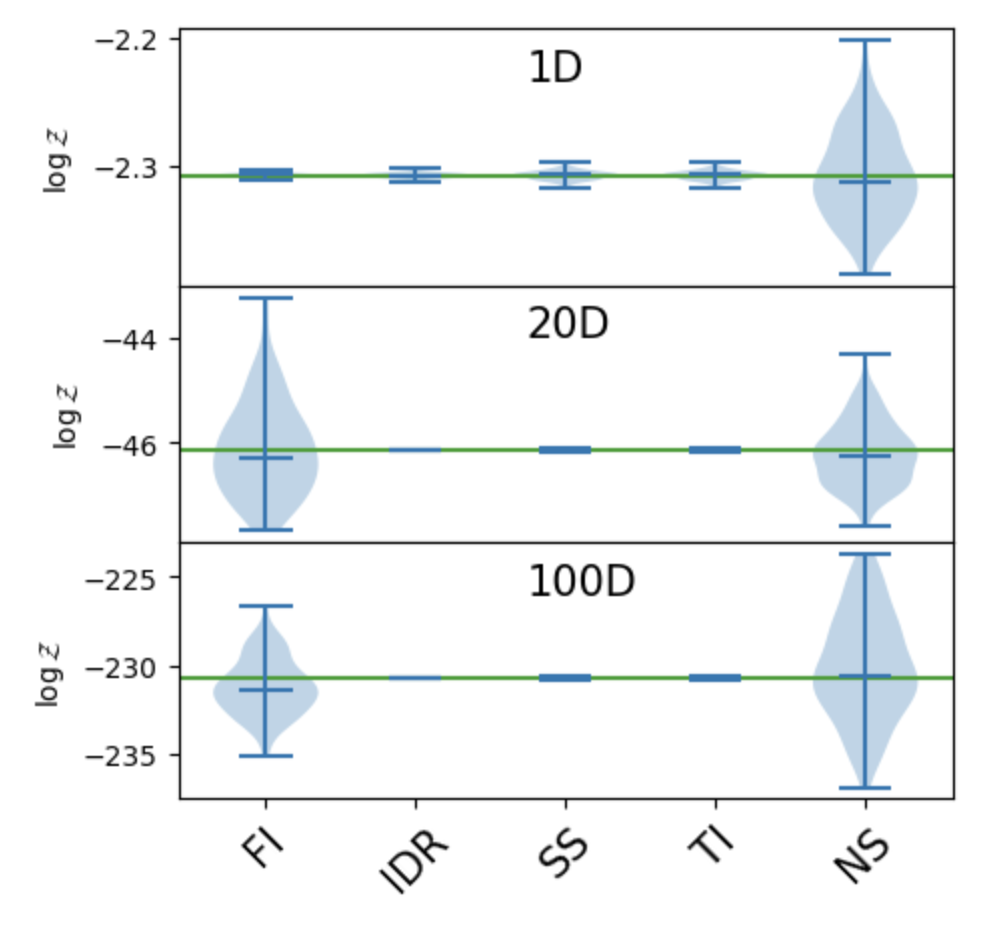
\includegraphics[width=0.5\linewidth]{pictures/FI_simulation.png}
    \caption{\avi{Change this to a hist?}}
    \label{fig:enter-label}
\end{figure}


\subsection{\label{subsec:LIGO} LIGO merger}
\avi{I will edit this}
\avi{Describe injection (what SNR, data, signal)}
\avi{Describe the sampler}


\begin{figure}[h]
\caption{A comparison of the FI, NS and SS $\ln \mathcal{L}$ using GW150914 data: The box plot displays the FI... The horizontal orange and green bars show the NS and SS... }
\centering
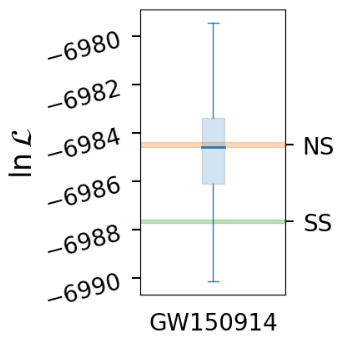
\includegraphics[width=0.3\textwidth]{pictures/GW150914.png}
\end{figure}

\subsection{\label{subsec:LISA} Simulated LISA SGWB}

Need Jason's plot here.



\section{\label{sec:discussion} Discussion}
Discuss some limitations of the FI method
Discuss future work -- to transform all posterior distributions into normal-like distributions.




\begin{acknowledgments}
Thank Rotiroti for discussions.

We wish to acknowledge the support of the author community in using
REV\TeX{}, offering suggestions and encouragement, testing new versions,
\dots.
\end{acknowledgments}

\appendix
\section{Appendixes}

\subsection{Mathematical details of equations \eqref{eqn: FI Exp asymptotic} and \eqref{eqn: FI Exp Dirichlet Integral}}
\label{subsec: maths details of the FI Exp example}
\subsubsection{Laplace transform of the sinc function and its Taylor series for equation \eqref{eqn: FI Exp asymptotic}}
\begin{proof}
We need to show that
\begin{equation*}
    \lambda \mathcal{L}\left\{\frac{\sin(R\theta)}{\theta} \right\} = \lambda \arctan\left(\frac{R}{\lambda}\right) \sim R.
\end{equation*}

As defined in section 3.2 of \cite{rotiroti2022computing}, the sine integral function is defined as
\begin{equation*}
    \text{Si}(z) = \int_0^z \frac{\sin(t)}{t} dt.
\end{equation*}
The integrand inside the sine integral function is called the sinc function. The integrand in equation \eqref{eqn: FI Exp asymptotic} is not quite a sinc function, but it is close enough for equation \eqref{eqn: FI Exp asymptotic} to be solved using the same steps as the ones to compute the Laplace transform on sinc function. Now
\begin{equation} \label{eqn: Laplace transform eta function}
    \mathcal{L}\left\{\frac{\sin(R\theta)}{\theta}\right\} = \int_0^\infty \frac{\sin(R\theta)}{\theta} e^{-\lambda \theta} d\theta =: \eta(R).
\end{equation}
Then using integration by parts,
\begin{align*}
    & \hspace{0.5cm} \eta'(R) \\
    & = \int_0^\infty e^{-\lambda \theta} \cos(R\theta) d\theta\\
    & = \left[\frac{e^{-\lambda\theta}}{-\lambda}\cos(R\theta) \right]_0^\infty - \int_0^\infty \frac{e^{-\lambda\theta}}{-\lambda}[-R\sin(R\theta)]d\theta \\
    & = \left[0-\frac{cos(0)}{-\lambda} \right] - \frac{R}{\lambda}\int_0^\infty e^{-\lambda\theta}\sin(R\theta)d\theta\\
    & = \frac{1}{\lambda} - \frac{R}{\lambda}\left\{\left[\frac{e^{-\lambda\theta}}{-\lambda}\sin(R\theta) \right]_0^\infty - \int_0^\infty \frac{e^{-\lambda\theta}}{-\lambda}R\cos(R\theta)d\theta \right\}\\
    & = \frac{1}{\lambda} - \frac{R}{\lambda}\left[0 - 0 + \frac{1}{\lambda}\int_0^\infty e^{-\lambda\theta}R\cos(R\theta) d\theta \right] \\
    & = \frac{1}{\lambda} - \frac{R^2}{\lambda^2}\int_0^\infty e^{-\lambda\theta} \cos(R\theta) d\theta \\
    & = \frac{1}{\lambda} - \frac{R^2}{\lambda^2} \eta'(R)\\
    & \implies \eta'(R) = \frac{\frac{1}{\lambda}}{1 + \left(\frac{R}{\lambda} \right)^2}\\
    & \implies \eta(R) = \int \frac{\frac{1}{\lambda}}{1 + \left(\frac{R}{\lambda} \right)^2} dR = \arctan\left(\frac{R}{\lambda} \right) + C
\end{align*}
By equation \eqref{eqn: Laplace transform eta function}, $\eta(0) = 0$. Thus,
\begin{equation*}
    C = \eta(0) - \arctan\left(\frac{0}{\lambda} \right) = 0,
\end{equation*}
so
\begin{equation} \label{eqn: Laplace=eta=arctan conclusion}
    \mathcal{L}\left\{\frac{\sin(R\theta)}{\theta}\right\} = \eta(R) = \arctan\left(\frac{R}{\lambda} \right).
\end{equation}
The Laplace transform of a sinc function can be obtained from equation \eqref{eqn: Laplace=eta=arctan conclusion} by substituting $R=1$.

Next, we need to show that $\lambda \arctan\left(\frac{R}{\lambda} \right) \sim R$. To see this, we first take the Taylor series of $\arctan(t)$, such that
\begin{equation*}
    \arctan(t) = \sum_{k = 0}^\infty (-1)^k \frac{t^{2k+1}}{2k+1}, \; \forall t \in (-1, 1).
\end{equation*}
See, for example, section 2 in \cite{nimbran2015taylor}. Also, we note that $\displaystyle \frac{R}{\lambda} \in [0, 1)$ as $\lambda \to \infty$. This gives, $\displaystyle \forall \left(\frac{R}{\lambda}\right) \in (-1, 1)$,
\begin{align*}
    & \arctan\left(\frac{R}{\lambda} \right)
    = \frac{R}{\lambda} - \frac{1}{3}\left[\frac{R}{\lambda} \right] + \mathcal{O}\left[\left(\frac{R}{\lambda} \right)^5 \right] \\
    \implies & \lambda \arctan\left(\frac{R}{\lambda} \right) = \lambda \frac{R}{\lambda} + \lambda \mathcal{O}\left[\left(\frac{R}{\lambda} \right)^3 \right] \sim \lambda \frac{R}{\lambda} = R.
\end{align*}
\end{proof}
\subsubsection{Dirichlet integral for equation \eqref{eqn: FI Exp Dirichlet Integral}}
\begin{proof}
    For $\chi := R\theta$, we need to show
    \begin{equation*}
        \text{Si}(\infty) = \frac{\pi}{2},
    \end{equation*}
    where
    \begin{align*}
        & \int_0^\infty \frac{\sin(R\theta)}{\theta} d\theta
        = \int_0^\infty \frac{\sin(\chi)}{\frac{\chi}{R}} \bigg|\frac{d\theta}{d\chi}\bigg| d\chi \\
        = & R \int_0^\infty \frac{\sin(\chi)}{\chi} \bigg|\frac{1}{R}\bigg| d\chi
        =: \text{Si}(\infty).
    \end{align*}
    Note that this sine integral function at infinity is also known as Dirichlet integral.
    Using Fubini's theorem,
    \begin{align} \label{eqn: Fubini's theorem for sine function at infinity}
        & \int_0^\infty\left[\int_0^\infty e^{-\lambda\chi}\sin(\chi)d\lambda\right]d\chi \\
        = & \int_0^\infty\left[\int_0^\infty e^{-\lambda\chi}\sin(\chi)d\chi\right]d\lambda.
    \end{align}
    Then for the left-hand side of equation \eqref{eqn: Fubini's theorem for sine function at infinity},
    \begin{align} \label{eqn: Fubini LHS}
        & \int_0^\infty e^{-\lambda\chi}\sin(\chi)d\lambda = \left[-e^{-\lambda\chi}\frac{\sin(\chi)}{\chi} \right]_{\lambda = 0}^\infty \\
        = & 0 + e^0\frac{\sin(\chi)}{\chi} = \frac{\sin(\chi)}{\chi}.
    \end{align}
    The right-hand side of equation \eqref{eqn: Fubini's theorem for sine function at infinity} is the Laplace transform of a sine function, which gives
    \begin{equation} \label{eqn: Fubini RHS}
        \int_0^\infty e^{-\lambda\chi}\sin(\chi)d\chi \\
        = \mathcal{L}\{\sin(\chi)\} = \frac{1}{\lambda^2 + 1}.
    \end{equation}
    Now substituting equations \eqref{eqn: Fubini LHS} and \eqref{eqn: Fubini RHS} into equation \eqref{eqn: Fubini's theorem for sine function at infinity}, one gets
    \begin{align*}
        & \text{Si}(\infty) = \int_0^\infty\left[\frac{\sin(\chi)}{\chi}\right]d\chi = \int_0^\infty\left[\frac{1}{\lambda^2 + 1}\right]d\lambda \\
        = & [\arctan(\lambda)]_0^\infty
        = \lim_{\lambda \uparrow \infty}\arctan(\lambda) - 0 = \frac{\pi}{2}.
    \end{align*}
\end{proof}

\subsection{Proof of theorem \ref{theorem: FI integral windows}}
\begin{proof}
    Let $\displaystyle J_\epsilon(\theta; x) := \int_{-\infty}^\infty \cos[s(x-\theta)]h_\epsilon(s)ds$ denote the inner integral of equation \eqref{eqn: integral window h(s)}. Part 1. follows the original version of FI estimator.

    Part 2: Let $t := s^2$. Then for $s > 0$, $s = \sqrt{t}$ and $\frac{ds}{dt} = \frac{1}{2\sqrt{t}}$. Both $s \mapsto \cos[s(x - \theta)]$ and $\displaystyle h_\tau(s) = e^{-s^2\tau}$ are even functions of $s$, so the inner integral of equation \eqref{eqn: integral window h(s)} becomes
    \begin{align*}
        J_\tau(\theta; x) = & \int_{-\infty}^\infty \cos[s(x - \theta)]e^{-s^2\tau}ds \\
        = & 2\int_0^\infty \cos[s(x - \theta)]e^{-s^2\tau}ds \\
        = & 2\int_0^\infty \cos[\sqrt{t}(x - \theta)]e^{-t\tau}\frac{1}{2\sqrt{t}}dt \\
        = & \mathcal{L}\left\{\frac{\cos[\sqrt{t}(x - \theta)]}{\sqrt{t}} \right\} \\
        = & \frac{\sqrt{\pi}e^{-\frac{(x - \theta)^2}{4\tau}}}{\sqrt{\tau}} = 2\pi\frac{\sqrt{\sigma^2}}{\sqrt{2\pi}}e^{-\frac{\sigma^2(x - \theta)^2}{2}} \\
        = & 2\pi p_\text{Norm}(\theta; \text{mean} = x, \text{var} = \frac{1}{\sigma^2} = 2\tau),
    \end{align*}
    where $\tau = \frac{1}{2\sigma^2}$ is twice of the normal-kernel precision parameter in $\displaystyle h_\tau(s) = e^{-s^2\tau} = e^{-\frac{s^2}{2\sigma^2}}$, but then it becomes half of the variance parameter in the resulting $p_\text{Norm}$ in $J_\tau(\theta; x)$. Finally, as $\tau \to 0$ makes $\displaystyle h_\tau(s) = e^{-s^2\tau}$ converge to $h(s) = 1$, from equation \eqref{eqn: integral window h(s)}, the estimating equation of the target density $p$ is given by
    \begin{align*}
        p(x) & = \frac{1}{2\pi} \lim_{\tau \to 0} \int_{-\infty}^\infty J_\tau(\theta; x) p(\theta)d\theta \\
        & = \lim_{\tau \to 0} \int_{-\infty}^\infty p_\text{Norm}(\theta; \text{mean} = x, \text{var} = 2\tau) p(\theta)d\theta,
    \end{align*}
    yielding the density estimator
    \begin{equation*}
        \hat{p}_n(x) = \frac{1}{n} \sum_{i = 1}^n p_\text{Norm}(\theta^{(i)}; \text{mean} = x, \text{var} = 2\tau)
    \end{equation*}
    for any reference point $x \in \Omega$ and $\tau$ a small positive value.

    Part 3: Since both $s \mapsto \cos[s(x - \theta)]$ and the double-exponential kernel $h_\tau(s) = e^{-|s|\tau}$ are even functions of $s$,
    \begin{align*}
        J_\tau(\theta, x) & = \int_{-\infty}^\infty \cos[s(x - \theta)]e^{-|s|\tau}ds \\
        & = 2\int_0^\infty \cos[s(x - \theta)]e^{-s\tau}ds \\
        & = 2 \mathcal{L}\{\cos[s(x - \theta)]\} \\
        & = 2\pi \left\{\frac{1}{\pi}\frac{\tau}{\tau^2 + (x - \theta)^2}\right\} \\
        & = 2\pi p_\text{Cauchy}(\theta, \text{location} = x, \text{scale} = \tau).
    \end{align*}
    Similar to part 2, the density estimator is
    \begin{equation*}
        \hat{p}_n(x) = \frac{1}{n} \sum_{i = 1}^n p_\text{Cauchy}(\theta^{(i)}; \text{location} = x, \text{scale} = \tau)
    \end{equation*}
    for any reference point $x \in \Omega$ and $\tau$ a small positive value.

    Part 4: Since both $s \mapsto \cos[s(x - \theta)]$ and the triangular kernel $\displaystyle h_R(s) = (1 - \frac{|s|}{R}) \mathbbm{1}[-R < s < R]$ are even functions of $s$,
    \begin{align*}
        J_R(\theta, x) & = \int_{-\infty}^\infty \cos[s(x - \theta)](1 - \frac{|s|}{R}) \mathbbm{1}[-R < s < R]ds \\
        & = 2 \int_0^R \cos[s(x - \theta)](1 - \frac{s}{R}) ds \\
        & = 2\left[\frac{\sin[s(x - \theta)]}{x - \theta}(1 - \frac{s}{R}) \right]^R_{s = 0} \\
        & \hspace{1cm} + 2\frac{1}{R(x - \theta)}\int_0^R \sin[s(x - \theta)]ds \\
        & = 2\left\{0+\frac{1}{R(x - \theta)} \left[-\frac{\cos(s(x - \theta)}{x - \theta} \right]^R_{s = 0} \right\} \\
        & = 2\frac{1}{R(x - \theta)^2}\{1 - \cos[R(x - \theta)]\}.
    \end{align*}
    As $R \to \infty$ makes $\displaystyle h_R(s) = (1 - \frac{|s|}{R}) \mathbbm{1}[-R < s < R]$ converge to $h(s) = 1$, the density estimation equation is
    \begin{align*}
        p(x) & = \frac{1}{2\pi} \lim_{R \to \infty} \int_{-\infty}^\infty J_R(\theta; x) p(\theta)d\theta \\
        & = \frac{1}{\pi} \lim_{R \to \infty} \int_{-\infty}^\infty \frac{1 - \cos[R(x - \theta)]}{R(x - \theta)^2} p(\theta) d\theta
    \end{align*}
    and the corresponding density estimator
    \begin{equation*}
        \hat{p}_n(x) = \frac{1}{n\pi} \sum_{i = 1}^n \frac{1}{R(x - \theta^{(i)})^2}\{1 - \cos[R(x - \theta^{(i)})]\}
    \end{equation*}
    for any reference point $x \in \Omega$ and a fixed large $R$.

    Part 5: Since both the Epanechnikov kernel $\displaystyle h_R(s) = (1 - \frac{s^2}{R^2}) \mathbbm{1}[-R < s < R]$ and $s \mapsto \cos[s(x - \theta)]$ are even functions of $s$,
    \begin{align*}
        J_R(\theta, x) & = \int_{-\infty}^\infty \cos[s(x - \theta)](1 - \frac{s^2}{R^2}) \mathbbm{1}[-R < s < R]ds \\
        & = 2 \int_0^R \cos[s(x - \theta)](1 - \frac{s^2}{R^2}) ds \\
        & = 2\left[\frac{\sin(s(x - \theta)}{x - \theta}(1 - \frac{s^2}{R^2}) \right]^R_{s = 0} \\
        & \hspace{1cm} -2\int_0^R \frac{\sin[s(x - \theta)]}{x - \theta}\left(-\frac{2s}{R^2} \right) ds \\
        & = 0 + \frac{4}{R^2(x - \theta)} \left[\frac{-\cos[s(x - \theta)]}{x - \theta}s \right]^R_{s = 0} \\
        & \hspace{1cm} - \frac{4}{R^2(x - \theta)} \int_0^R \frac{-\cos[s(x - \theta)]}{x - \theta} ds \\
        & = -\frac{4}{R^2(x - \theta)^2}\cos[R(x - \theta)]R \\
        & \hspace{1cm} + \frac{4}{R^2(x - \theta)^2}\left[\frac{\sin([s(x - \theta)]}{x - \theta} \right]^R_{s = 0} \\
        & = \frac{4\left\{\frac{\sin[R(x - \theta)]}{x - \theta} - R\cos[R(x - \theta)] \right\}}{R^2(x - \theta)^2}.
    \end{align*}
    Similar to part 4, the density estimator is then given by
    \begin{equation*}
        \hat{p}_n(x) = \frac{1}{n\pi} \sum_{i = 1}^n \frac{2\left\{\frac{\sin[R(x - \theta^{(i)})]}{x - \theta^{(i)}} - R\cos[R(x - \theta^{(i)})] \right\}}{R^2(x - \theta^{(i)})^2}
    \end{equation*}
    for any reference point $x \in \Omega$ and a fixed large $R$.
\end{proof}

\subsection{Proof of remark \ref{remark: triangle inequality in aFI}}

\begin{proof}
    We need to compare the two candidate estimators on both sides of the inequality in remark \ref{remark: triangle inequality in aFI} and decide which one is consistent with the original FI density estimator. To compare the two estimators, we compare their corresponding estimating equations,
    \begin{equation*}
         m_1(\xbold) := \bigg|\int_\R \prod_{j = 1}^d \frac{\sin(R_j(x_j - \theta_j))}{x_j - \theta_j} p(\btheta)d\btheta\bigg|
    \end{equation*}
    and
    \begin{equation*}
        m_2(\xbold) := \int_\R \bigg|\prod_{j = 1}^d \frac{\sin(R_j(x_j - \theta_j))}{x_j - \theta_j} p(\btheta)d\btheta\bigg|.
    \end{equation*}
    We compare the estimating equations by observing which one can be reduced to the original FI estimator at the $R$ values where the density estimate is positive.

    Let
    \begin{equation*}
        a(\xbold) := \int_\R \prod_{j = 1}^d \frac{\sin(R_j(x_j - \theta_j))}{x_j - \theta_j} p(\btheta)d\btheta,
    \end{equation*}
    which is the original FI density estimating equation. Let $I := \{\xbold \in \R^d | a(\xbold) \ge 0\}$ be the parameter space where the original FI is density estimating equation is positive. Then, the improved FI must agree with the original FI on $I$. Furthermore, let
    \begin{equation*}
        b(\xbold) := \int_\R \prod_{j = 1}^d \frac{\sin(-R_j(x_j - \theta_j))}{x_j - \theta_j} p(\btheta)d\btheta,
    \end{equation*}
    the negative FI density estimating equation. Then
    \begin{equation*}
        m_1(\xbold) = a(\xbold)\mathbbm{1}[a(\xbold) \ge 0] + b(\xbold) \mathbbm{1}[a(\xbold) < 0].
    \end{equation*}
    Hence, on the set $I$,
    \begin{align*}
        & m_1(\xbold)\mathbbm{1}[\xbold \in I] = m_1(\xbold)\mathbbm{1}[a(\xbold) \ge 0] \\
        = & [a(\xbold)\mathbbm{1}[a(\xbold) \ge 0] + b(\xbold) \mathbbm{1}[a(\xbold) < 0]]\mathbbm{1}[a(\xbold) \ge 0] \\
        = & a(\xbold)\mathbbm{1}[a(\xbold) \ge 0] = a(\xbold)\mathbbm{1}[\xbold \in I]
    \end{align*}

    Then we consider $m_2(\xbold)$. For any integrable function $k$, define $k^+(x) := |k(x)|\mathbbm{1}[k(x) \ge 0]$ and $k^-(x) := |k(x)|\mathbbm{1}[k(x) < 0]$. Then one can derive $k(x) = k^+(x) - k^-(x)$ and $|k(x)| = k^+(x) + k^-(x)$. Define
    \begin{equation*}
        r(\xbold, \btheta) := \prod_{j = 1}^d \frac{\sin(R_j(x_j - \theta_j))}{x_j - \theta_j} p(\btheta).
    \end{equation*}
    Then $\forall \mathbf{j} \in I$,
    \begin{align*}
        & m_2(\mathbf{j}) = \int_\R |r(\mathbf{j}, \btheta)|p(\btheta)d\btheta \\
        = & \int_\R [r^+(\mathbf{j}, \btheta) + r^-(\mathbf{j}, \btheta)]p(\btheta)d\btheta \\
        = & \int_\R [r^+(\mathbf{j}, \btheta) - r^-(\mathbf{j}, \btheta)]p(\btheta)d\btheta + 2\int_\R r^-(\mathbf{j}, \btheta)p(\btheta)d\btheta \\
        = & \int_\R r(\mathbf{j}, \btheta)p(\btheta)d\btheta + 2\int_\R r^-(\mathbf{j}, \btheta)p(\btheta)d\btheta \\
        = & a(\mathbf{j}) + 2\int_\R r^-(\mathbf{j}, \btheta)p(\btheta)d\btheta \ge a(\mathbf{j}).
    \end{align*}
Therefore, $m_1(\xbold)$ should be the estimating equation, not $m_2(\xbold)$.
\end{proof}

\subsection{Proof of proposition \ref{prop: FI Gaussian bias}}
\begin{proof}
    First, we denote the absolute FI estimator based on one observation to be $\hat{p}_{\text{1}}$, and the absolute FI estimator based on a sample of size $n$ to be $\hat{p}_{n}$.

    Let the precision parameter be $s_j := := \frac{1}{2\sigma_j^2}$, and set $u_j := \theta_j^2$, hence $du_j = 2\sqrt{u}d\theta_j$. Then the FI estimator of density based on a single Gaussian$(\mathbf{0},
    \boldsymbol{\sigma})$ observation is given by
    \begin{align*}
        & \E[\hat{p}_{\text{1}}(\mathbf{0})] \\
        = & \int_{\btheta = -\boldsymbol{\infty}}^{\boldsymbol{\infty}}\bigg|\prod_{j = 1}^d \frac{1}{\pi} \frac{\sin[R_j(0 - \theta_j)]}{0 - \theta}\bigg| p(\btheta)d\btheta \\
        = & \prod_{j = 1}^d \int_{\theta_j = -\infty}^\infty\bigg|\frac{1}{\pi} \frac{-\sin[R_j\theta_j]}{ - \theta_j}\bigg| p(\theta_j) d\theta_j \\
        = & \prod_{j = 1}^d \int_{\theta_j = -\infty}^\infty\frac{1}{\pi\sqrt{2\pi}\sigma_j}\bigg| \frac{\sin[R_j\theta_j]}{\theta_j}\bigg| e^{-\frac{\theta_j^2}{2\sigma_j^2}} d\theta_j \\
        = & \prod_{j = 1}^d \frac{\sqrt{2s_j}}{\pi\sqrt{2\pi}}2\int_{\theta_j = 0}^\infty \bigg| \frac{\sin[R_j\theta_j]}{\theta_j}\bigg| e^{-s_j\theta_j^2} d\theta_j \\
        = & \prod_{j = 1}^d \frac{2\sqrt{s_j}}{\pi\sqrt{\pi}}\int_{u_j = 0}^\infty \bigg| \frac{\sin[R_j\sqrt{u_j}]}{\sqrt{u_j}}\bigg| e^{-s_ju_j} \frac{1}{2\sqrt{u_j}}du_j \\
        = & \prod_{j = 1}^d \frac{\sqrt{s_j}}{\pi\sqrt{\pi}} \mathcal{L}_{u_j}\left\{\bigg|\frac{\sin(R_j\sqrt{u_j})}{u_j} \bigg| \right\}(s_j) \\
        = & \prod_{j = 1}^d \frac{\sqrt{s_j}}{\pi\sqrt{\pi}} \pi \erf\left(\frac{R_j}{2\sqrt{s_j}} \right) \\
        = & \prod_{j = 1}^d \frac{1}{\pi\sqrt{2\pi}\sigma_j} \pi \erf\left(\frac{R_j\sqrt{2}\sigma_j}{2} \right)
    \end{align*}
    Also note that, the FI estimators based on a sample of size $n$ and a single observation has the relationship that
    \begin{align*}
    \hat{p}_{n}(\mathbf{x}) & = \bigg|\frac{1}{n\pi^d}\sum_{i = 1}^n \prod_{j = 1}^d \frac{\sin(R_j(x_j - \theta_j^{(i)}))}{x_j - \theta_j^{(i)}}\bigg| \\
    & \le \frac{1}{n\pi^d}\sum_{i = 1}^n \bigg|\prod_{j = 1}^d \frac{\sin(R_j(x_j - \theta_j^{(i)}))}{x_j - \theta_j^{(i)}}\bigg|\\
    & = \frac{\sum_{i=1}^n\hat{p}_{\text{1}}(\mathbf{x})}{n},
    \end{align*}
    hence
    $$
    \E[\hat{p}_{n}(\mathbf{x})] \le \E\left[\frac{\sum_{i=1}^n\hat{p}_{\text{1}}(\mathbf{x})}{n}\right] = \E[\hat{p}_{\text{FI}1}(\mathbf{x})].
    $$
    This means that, for any sample with size $n$,
    \begin{align*}
        & \text{bias}(\hat{p}_n(\mathbf{0})) \\
        = & \E[\hat{p}_{n}(\mathbf{0}) - p_{\text{N}(\mathbf{0}, \boldsymbol{\sigma})}(\mathbf{0})] \\
        \le & \E[\hat{p}_{\text{1}}(\mathbf{x})] - p_{\text{N}(\mathbf{0}, \boldsymbol{\sigma})}(\mathbf{0})\\
        = & \prod_{j=1}^d \frac{1}{\sqrt{2\pi}\sigma_j}\left\{\erf\left[\frac{R_j \sqrt{2}\sigma_j}{2} \right]-1 \right\} \le 0
    \end{align*}
\end{proof}


% The \nocite command causes all entries in a bibliography to be printed out
% whether or not they are actually referenced in the text. This is appropriate
% for the sample file to show the different styles of references, but authors
% most likely will not want to use it.
%\nocite{*}

\bibliography{my_bib}% Produces the bibliography via BibTeX.

\end{document}
%
% ****** End of file apssamp.tex ******

